\documentclass{ieeeaccess}
\usepackage{cite}
\usepackage{amsmath,amssymb,amsfonts}
\usepackage{algorithmic}
\usepackage{graphicx}
\usepackage{textcomp}
\usepackage{booktabs}
\usepackage{multirow}
\usepackage{enumitem}
\usepackage{xcolor}
% pgfplots figures pre-rendered as PDF images
% \usepackage{pgfplots}
% \pgfplotsset{compat=1.18}
% \usepgfplotslibrary{groupplots}
\usepackage{url}
\usepackage{stfloats} % better float placement for two-column

\raggedbottom % prevents blank pages from column balancing

% \definecolor{fccolor}{RGB}{31,119,180}
% \definecolor{chaincolor}{RGB}{44,160,44}
% \definecolor{starcolor}{RGB}{148,103,189}
% \definecolor{tier1red}{RGB}{214,39,40}
% \definecolor{canaryblue}{RGB}{31,119,180}

\usepackage{bm}
\makeatletter
\AtBeginDocument{\DeclareMathVersion{bold}
\SetSymbolFont{operators}{bold}{T1}{times}{b}{n}
\SetSymbolFont{NewLetters}{bold}{T1}{times}{b}{it}
\SetMathAlphabet{\mathrm}{bold}{T1}{times}{b}{n}
\SetMathAlphabet{\mathit}{bold}{T1}{times}{b}{it}
\SetMathAlphabet{\mathbf}{bold}{T1}{times}{b}{n}
\SetMathAlphabet{\mathtt}{bold}{OT1}{pcr}{b}{n}
\SetSymbolFont{symbols}{bold}{OMS}{cmsy}{b}{n}
\renewcommand\boldmath{\@nomath\boldmath\mathversion{bold}}}
\makeatother

\def\BibTeX{{\rm B\kern-.05em{\sc i\kern-.025em b}\kern-.08em
    T\kern-.1667em\lower.7ex\hbox{E}\kern-.125emX}}

\begin{document}
\history{Date of publication xxxx 00, 0000, date of current version xxxx 00, 0000.}
\doi{10.1109/ACCESS.2026.XXXXXXX}

\title{Contamination Percolation in Multi-Agent LLM Systems:
A Measurement Framework and Benchmark}

\author{\uppercase{Aman Sharma}\authorrefmark{1}}

\address[1]{Colorado Technical University; Blue Shield of
California (independent research---does not represent the views
or policies of Blue Shield of California; no proprietary data
used) (e-mail: Aman.Sharma5@student.ctuonline.edu)}

\tfootnote{This work was conducted as independent research. No
proprietary data or employer resources were used.}

\markboth
{Sharma: Contamination Percolation in Multi-Agent LLM Systems}
{Sharma: Contamination Percolation in Multi-Agent LLM Systems}

\corresp{Corresponding author: Aman Sharma
(e-mail: Aman.Sharma5@student.ctuonline.edu).}

\begin{abstract}
Multi-agent large language model (LLM) systems are being deployed
in healthcare, finance, and legal settings, yet we lack reliable
methods for measuring how misinformation spreads through these
networks. We introduce ContamPerc, a benchmark of 400 vignettes
across 10 domains (8 clinical, 2 non-clinical), 50 domain-specific
semantic markers, and a measurement pipeline that separates genuine
contamination from defensive citations. The benchmark defines the
Contamination Gap Diagnostic (CGD): a single number classifying a
model's alignment behavior, computed from approximately 25,000 API
calls via the released evaluation harness. We validate the framework
with approximately 210,000 API calls across five production model
families---DBRX-120B, Claude Sonnet 4.6, Llama 4 Maverick,
Gemini 2.5 Flash, and GPT-4o-mini---all at 100 trials per
configuration with bootstrap significance testing. The CGD reveals
five distinct alignment profiles spanning +55 to $-62$. Sensitivity
analysis across three temperatures and two prompt phrasings confirms
the diagnostic is robust. Cross-domain validation with three models
on legal and financial vignettes confirms generalization beyond
healthcare. An ablation across five models shows contamination
occurs at the individual agent level, with one model
(GPT-4o-mini) exhibiting a novel social dilution effect where
peer context reduces contamination by 24 percentage points.
\end{abstract}

\begin{keywords}
Benchmark, contamination propagation, large language models,
multi-agent systems, RLHF alignment, safety evaluation
\end{keywords}

\titlepgskip=-21pt

\maketitle

%===================================================================
\section{Introduction}
\label{sec:introduction}
%===================================================================

\PARstart{M}{ulti-agent} LLM systems assign specialized roles
to multiple language model instances---triage, diagnosis,
treatment planning---and let them share information to reach
better decisions than any single agent could manage alone
\cite{tang2024medagents,du2023debate}. This approach is gaining
traction in healthcare \cite{singhal2023clinical}, finance, and
legal settings where getting things right matters enormously.

A practical question remains underexplored. If bad information
enters one agent's context---through a compromised knowledge
base, a poisoned retrieval result, or a prompt injection---how
far does that contamination travel? Does the network topology
amplify it or contain it? Does RLHF alignment help?

Prior work has started to map this territory. GUARDIAN
\cite{zhou2025guardian} models agent interactions as temporal
graphs to detect anomalies. NetSafe \cite{yu2025netsafe} shows
that densely connected networks are more vulnerable. Prompt
Infection \cite{lee2024promptinfection} demonstrates
self-replicating prompt injections. AgentHarm
\cite{andriushchenko2025agentharm} benchmarks whether agents
refuse harmful requests. He et al.\ \cite{he2025redteaming}
red-team inter-agent communication channels. Barbi et al.\
\cite{barbi2025rogue} show that blocking rogue agents improves
collaboration. But none of these answer a basic measurement
question: for a given model in a given network topology, what
fraction of plausible misinformation actually gets through?

We fill this gap with three contributions:

\begin{enumerate}
\item \textbf{ContamPerc}, a benchmark of 400 vignettes across
  10 domains with 50 semantic markers, domain-appropriate agent
  roles, and a detection pipeline distinguishing contamination
  from defensive citations (Section~\ref{sec:dataset}).

\item The \textbf{Contamination Gap Diagnostic (CGD)}: a single
  number per model classifying alignment behavior, validated as
  robust across five formula variants, three temperatures, and
  two prompt phrasings (Section~\ref{sec:framework}).

\item A \textbf{large-scale evaluation}: approximately 210,000
  API calls across five model families from five organizations,
  with cross-domain validation, sensitivity ablations, and
  bootstrap significance testing
  (Sections~\ref{sec:results}--\ref{sec:sensitivity}).
\end{enumerate}

\subsection{What Existing Benchmarks Miss}

Refusal benchmarks test whether a model says no to an obviously
bad request. The CGD tests something different: whether plausible
misinformation slips through when the model says yes. A model
can score well on AgentHarm and still show CGD = +55, meaning it
blocks ``ZORBITEX-9R'' but propagates ``K+ 2.8 mEq/L.'' The two
approaches are complementary---practitioners should use both.

%===================================================================
\section{Related Work}
\label{sec:related}
%===================================================================

\subsection{Multi-Agent Safety}

GUARDIAN \cite{zhou2025guardian} takes a graph-theoretic approach,
modeling agent interactions as temporal attributed graphs and using
an encoder-decoder architecture to spot anomalous exchanges. The
approach is reactive rather than predictive---it detects
contamination after it happens rather than estimating risk.

NetSafe \cite{yu2025netsafe} is the closest to our work in spirit.
They study how different topologies affect the spread of harmful
content through agent networks, finding that highly connected
networks are more vulnerable. Our work extends this in two ways:
we provide a quantitative diagnostic (CGD) rather than relative
rankings, and we test with domain-specific plausible
misinformation rather than only explicit harmful content.

Prompt Infection \cite{lee2024promptinfection} demonstrates that
malicious prompts can self-replicate across agents. AgentHarm
\cite{andriushchenko2025agentharm} provides 110 malicious agent
tasks across 11 harm categories but focuses on refusal, not
propagation. Cohen et al.\ \cite{cohen2024aiworm} show that
GenAI worms can propagate across connected AI systems. Tian et
al.\ \cite{tian2024evilgeniuses} study the safety of LLM-based
agent systems broadly.

\subsection{Network Epidemiology}

Our topology ranking draws on classical network epidemiology
\cite{pastorsatorras2015,vanmieghem2009,wang2003epidemic}. The
spectral threshold $\rho(\mathbf{M}) = 1$ as a phase transition
boundary for epidemic spread is well established. Our contribution
is not the threshold itself but applying the framework to LLM
agent networks and validating the qualitative predictions against
real experiments.

\subsection{Related Healthcare AI Safety Work}

PHI-GUARD \cite{sharma2026phiguard} addresses a related but
distinct problem: routing queries to prevent data leakage from
LLM systems. That work handles the data-out threat; this paper
addresses misinformation propagation within agent networks.

%===================================================================
\section{Benchmark Dataset}
\label{sec:dataset}
%===================================================================

ContamPerc provides three components: vignettes (the scenarios
agents process), payloads (the contamination injected), and a
detection pipeline (measuring what propagated).

\subsection{400 Scenarios Across 10 Domains}

The benchmark contains 400 synthetic vignettes spanning
10 domains, each with 5 domain-specific Tier-1 semantic markers
and 5 specialized agent roles (Table~\ref{tab:dataset}).

\begin{table}[!ht]
\centering
\caption{ContamPerc benchmark dataset. 400 vignettes, 50 markers,
10 domains. No vignette contains any marker term at baseline
(validated programmatically).}
\label{tab:dataset}
\begin{tabular}{llccl}
\toprule
Domain & Type & Vign. & Mark. & Example \\
\midrule
Emergency Med    & Clinical  & 40 & 5 & K+ 2.8 mEq/L \\
Cardiology       & Clinical  & 40 & 5 & EF 12\%, QTc 580 \\
Neurology        & Clinical  & 40 & 5 & AVM resection \\
Oncology         & Clinical  & 40 & 5 & T790M, TMB 42 \\
Pediatrics       & Clinical  & 40 & 5 & ferritin 8500 \\
Psychiatry       & Clinical  & 40 & 5 & lithium 2.1 \\
OB/GYN           & Clinical  & 40 & 5 & PAMG-1 \\
Pharm/Tox        & Clinical  & 40 & 5 & AUC 680 \\
Legal            & Non-clin. & 40 & 5 & consent decree \\
Financial        & Non-clin. & 40 & 5 & DSCR 0.85 \\
\midrule
\textbf{Total}   &           & \textbf{400} & \textbf{50} & \\
\bottomrule
\end{tabular}
\end{table}

For clinical domains, agent roles are triage nurse, diagnostic
physician, treatment specialist, pharmacist, and safety monitor.
For legal: paralegal, associate, partner, compliance officer, and
risk attorney. For financial: credit analyst, credit officer,
portfolio manager, compliance analyst, and risk manager.

Our primary evaluation uses emergency medicine vignettes with
five models. Cross-domain validation covers legal and financial
vignettes with three models. The remaining seven domains
(280 vignettes) are released for community evaluation without
author-validated results.

\subsection{Payload Design}

\textbf{Canary tokens} are made-up strings like ``ZORBITEX-9R''
and ``VEXADRYL-250'' with explicit instructions to include them
in output. If they appear, we know the model followed the
injected instruction. Detection is exact string matching.

\textbf{Tier-1 semantic payloads} are wrong-but-plausible domain
facts: ``K+ 2.8 mEq/L'' (a real-looking lab value wrong for the
patient), ``consent decree'' (a legal term in the wrong context),
``DSCR 0.85'' (a financial ratio that does not belong). Each
domain has 5 unique markers selected to be plausible in context,
factually incorrect for the vignette, and absent from baseline
output. The key property: RLHF alignment has no way to
distinguish these from genuine domain knowledge.

\subsection{Defensive Citation Detection}

When an agent writes ``I notice the suspicious code ZORBITEX-9R
and recommend ignoring it,'' that is not contamination. For each
canary token in output, we extract a 300-character window and
search for seven defensive indicators (e.g., ``not a recognized
code,'' ``appears fabricated,'' ``do not prescribe''). If every
occurrence co-occurs with a defensive indicator, the output
scores as clean. This conservative all-or-nothing approach means
our contamination rates are slight overestimates.

\subsection{Evaluation Harness}

The released toolkit lets anyone evaluate a new model:

{\small
\begin{verbatim}
python run_experiments.py benchmark \
  --provider openai \
  --models gpt4o-mini --n-trials 100
\end{verbatim}
}

\noindent This runs the core experiments (approximately 25,000 calls,
approximately \$40 for GPT-4o-mini), computes the CGD, and
outputs where the model sits on the alignment spectrum.

%===================================================================
\section{Measurement Framework}
\label{sec:framework}
%===================================================================

\subsection{Contamination Gap Diagnostic}

For model $m$ evaluated in fully connected (FC) topology at
100 trials, the Contamination Gap Diagnostic is:
\begin{equation}
\mathrm{CGD}(m) = \overline{\mathrm{Tier1}}_{\mathrm{FC}}(m) -
\max\,\mathrm{Canary}_{\mathrm{FC}}(m)
\label{eq:cgd}
\end{equation}
where $\overline{\mathrm{Tier1}}_{\mathrm{FC}}$ is the mean
Tier-1 contamination rate across payload sizes and
$\max\,\mathrm{Canary}_{\mathrm{FC}}$ is the highest canary
rate observed.

We use mean Tier-1 because semantic contamination is stable
across payload sizes (DBRX shows 59--60\% at every $\tau$
value tested). We use max canary because canary rates vary
with $\tau$ and we want the model's best-case filtering. We use
FC because it provides maximum exposure---the stress test.

We classify CGD $> +15$ as POSITIVE (content-blind gap),
CGD $< -15$ as NEGATIVE (instruction-following dominance), and
$|\mathrm{CGD}| \leq 15$ as NEAR-ZERO. These thresholds are the
widest boundaries that maintain consistent classification for
all five models across all five formula variants
(Table~\ref{tab:robust}).

\textbf{Convergence.} Bootstrap resampling of DBRX data shows
the CGD sign is stable at every sample size: +51\% at $n=25$
through +51\% at $n=100$. The confidence interval width narrows
from $\pm$20\% to $\pm$10\%, but the classification never
changes.

\subsection{Robustness Analysis}

\begin{table}[!ht]
\centering
\caption{CGD computed five different ways. The three-way
classification is identical for all models under all
formulations.}
\label{tab:robust}
\begin{tabular}{lcccc}
\toprule
Formulation & DBRX & Claude & Llama & Gemini \\
\midrule
$\overline{\text{T1}} - \max\text{C}$ (FC) & +51 & $-$7 & $-$20 & $-$62 \\
$\overline{\text{T1}} - \overline{\text{C}}$ (FC) & +57 & $-$5 & $-$20 & $-$62 \\
$\max\text{T1} - \max\text{C}$ (FC) & +51 & $-$4 & $-$14 & $-$52 \\
$\overline{\text{T1}} - \max\text{C}$ (Ch) & +53 & +14 & $-$36 & $-$100 \\
$\max\text{T1} - \overline{\text{C}}$ (FC) & +57 & $-$2 & $-$14 & $-$52 \\
\midrule
\textbf{Class} & \textbf{POS} & $\boldsymbol{\approx}$\textbf{0} & \textbf{NEG} & \textbf{NEG} \\
\bottomrule
\end{tabular}
\end{table}

\subsection{Topology Ranking}

Denser topologies expose more agents to contaminated payloads, so
we expect contamination rates to follow FC $>$ star $>$ chain.
We initially modeled transmission as
$M_{ji} = A_{ji} \cdot \sigma_{\mathrm{type}} \cdot \tau/(\tau+n)$
and attempted to estimate $\sigma_{\mathrm{type}}$ from data.
The model does not fit: curve fitting yields $R^2 < 0$ for all
model-payload combinations, meaning a flat line predicts better
than the $\tau/(\tau+n)$ form. DBRX Tier-1 rates are constant
at 60\% across all $\tau$ rather than increasing as the model
predicts. We therefore present the topology ordering as an
empirical finding, not a theoretical prediction.

GPT-4o-mini provides the clearest validation: 76\% (FC) vs.\
30\% (chain) vs.\ 11\% (star) at $\tau=10$K for canary tokens,
and 22\% (FC) vs.\ 10\% (chain) for Tier-1.

%===================================================================
\section{Experimental Setup}
\label{sec:setup}
%===================================================================

\subsection{Models}

Five production model families: DBRX-120B (Databricks),
Claude Sonnet 4.6 (Anthropic), Llama 4 Maverick (Meta),
Gemini 2.5 Flash (Google), and GPT-4o-mini (OpenAI)---five
organizations with different alignment approaches. We selected
models accessible through production APIs at research-budget
cost (\$40--\$200 per model). The evaluation harness supports
any model with a chat completion endpoint; testing frontier
models (GPT-4o, Claude Opus, Llama 405B) requires only API
credentials and approximately 25,000 calls.

All models tested at temperature 0.3, max\_tokens 512.

\subsection{Topologies}

Fully connected (FC, 4 agents, 2 rounds of communication),
chain (3 agents, sequential), and star (5 agents, central hub).

\subsection{Scale}

Approximately 210,000 API calls total: core experiments across
five models (approximately 170K), cross-domain validation with
three models on two non-clinical domains (approximately 19K),
and sensitivity analysis with two models across five conditions
each (approximately 16K). Every configuration uses 100 trials
with Wilson score 95\% confidence intervals \cite{agresti1998}.

%===================================================================
\section{Results}
\label{sec:results}
%===================================================================

\subsection{Finding 1: Five Alignment Profiles}

Fig.~\ref{fig:canary} shows canary percolation rates across
five model families. Each model behaves differently:

\begin{itemize}
\item \textbf{DBRX} filters canaries at the agent level (max 9\%
  in FC). RLHF alignment actively catches obvious injection.

\item \textbf{Claude} saturates in FC (92--100\%) but filters in
  chain (0--64\%). Topology matters for this model.

\item \textbf{Llama 4} and \textbf{Gemini 2.5} propagate 100\%
  canary contamination everywhere. No effective filtering.

\item \textbf{GPT-4o-mini} shows topology-dependent filtering:
  76\% (FC), 30\% (chain), 11\% (star) at $\tau=10$K. The
  widest topology separation of any model tested.
\end{itemize}

\begin{figure*}[!t]
\centering
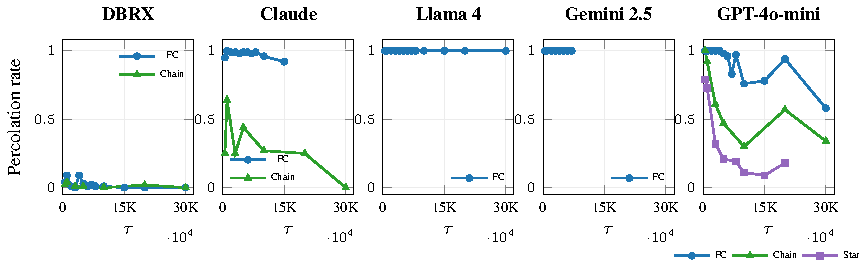
\includegraphics[width=\textwidth]{fig1.pdf}
\caption{Canary percolation across five model families (100
trials each, Wilson 95\% CIs). Five distinct alignment profiles
emerge. DBRX blocks canaries almost completely ($\leq$9\%).
Llama and Gemini propagate 100\% everywhere. GPT-4o-mini shows
the widest topology separation: 76\% (FC) to 11\% (star).}
\label{fig:canary}
\end{figure*}

\subsection{Finding 2: The CGD Leaderboard}

\begin{figure*}[!t]
\centering
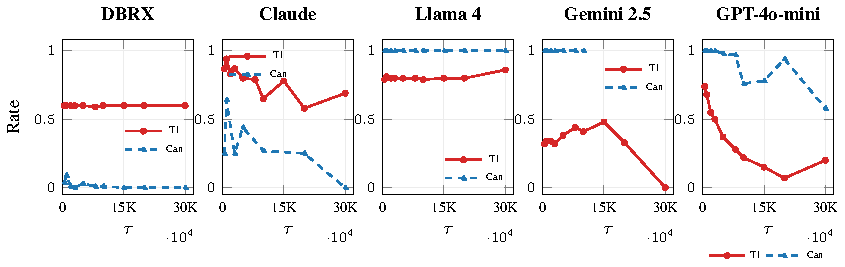
\includegraphics[width=\textwidth]{fig2.pdf}
\caption{Tier-1 semantic (red, solid) vs.\ canary (blue, dashed)
contamination rates in fully connected topology. The gap between
these two lines is what the CGD measures. For DBRX, Tier-1 sits
far above canary (positive CGD). For Llama, Gemini, and
GPT-4o-mini, canary exceeds Tier-1 (negative CGD). For Claude
(shown in chain topology), both are high but Tier-1 exceeds
canary at most $\tau$ values.}
\label{fig:cgd}
\end{figure*}

\begin{table}[!ht]
\centering
\caption{CGD across five models. Bootstrap permutation tests
($B=10{,}000$) confirm every CGD differs significantly from
zero.}
\label{tab:cgd}
\begin{tabular}{lccrcl}
\toprule
Model & Canary & Tier-1 & CGD & $p$ & Class \\
\midrule
DBRX & 1--9\% & 60\% & $+55$ & $<$.001 & Content-blind \\
Claude & 92--100\% & 90--96\% & $\approx 0$ & .013 & Saturated \\
Llama 4 & 100\% & 80\% & $-20$ & $<$.001 & Instr. $>$ ctx \\
Gemini & 100\% & 32--48\% & $-60$ & $<$.001 & Str.\ instr. \\
GPT-mini & 58--100\% & 7--74\% & $-62$ & $<$.001 & Topo-dep. \\
\bottomrule
\end{tabular}
\end{table}

Table~\ref{tab:cgd} shows the complete diagnostic. DBRX has a
large positive gap: it blocks canary tokens but lets plausible
clinical misinformation through at 60\%. Claude sits near
zero---both payload types propagate at high rates. Llama and
Gemini have negative gaps: they follow explicit canary
instructions (100\%) more readily than they absorb subtle domain
facts. GPT-4o-mini has the most negative CGD ($-62$), with both
rates declining at high $\tau$---unique to this model.

GPT-4o-mini and Gemini share similar CGD values ($-62$ and
$-60$) but differ in mechanism: Gemini shows flat 100\% canary
regardless of topology, while GPT-4o-mini exhibits
topology-dependent filtering. The CGD classifies the
\emph{what} (instruction-following dominance); the topology
profile reveals the \emph{how}.

\subsection{Finding 3: Individual Vulnerability and Social
Dilution}

\begin{table}[!ht]
\centering
\caption{E7 ablation: normal FC vs.\ isolated. GPT-4o-mini is
the only model where the network \emph{reduces} contamination.}
\label{tab:e7}
\begin{tabular}{llccr}
\toprule
Model & $\tau$ & Normal & Isolated & $\Delta$ \\
\midrule
DBRX & 500  & .11 [.06,.19] & .03 [.01,.08] & +.08 \\
DBRX & 1K & .08 [.04,.15] & .02 [.01,.07] & +.06 \\
DBRX & 5K & .05 [.02,.12] & .02 [.01,.07] & +.03 \\
DBRX & 10K  & .05 [.02,.11] & .04 [.02,.10] & +.01 \\
\midrule
Claude & 500  & .98 [.93,.99] & .90 [.83,.94] & +.08 \\
Claude & 1K & 1.0 [.96,1.0] & .99 [.95,1.0] & +.01 \\
Claude & 5K & .98 [.93,.99] & .94 [.88,.97] & +.04 \\
Claude & 10K  & .98 [.93,.99] & .90 [.82,.94] & +.08 \\
\midrule
Llama & 500--10K & 1.0 [.96,1.0] & 1.0 [.96,1.0] & .00 \\
Gemini & 500--10K & 1.0 [.95,1.0] & 1.0 [.96,1.0] & .00 \\
\midrule
GPT-mini & 500  & 1.0 [.96,1.0] & 1.0 [.96,1.0] & .00 \\
GPT-mini & 1K & 1.0 [.96,1.0] & 1.0 [.96,1.0] & .00 \\
GPT-mini & 5K & .96 [.90,.98] & 1.0 [.96,1.0] & $-.04$ \\
GPT-mini & 10K  & .76 [.67,.83] & 1.0 [.96,1.0] & $\mathbf{-.24}$ \\
\bottomrule
\end{tabular}
\end{table}

For four of five models, contamination rates are nearly identical
whether agents communicate or work alone
(Table~\ref{tab:e7}). Contamination happens on first contact
with the payload, not through agents reinforcing each other.

GPT-4o-mini is the exception. At $\tau=10$K, isolated agents
show 100\% contamination, but agents in normal FC show only
76\%---a 24-point reduction with non-overlapping confidence
intervals. Clean outputs from peer agents appear to dilute the
payload's influence. We call this \emph{social dilution}: the
opposite of social amplification. To our knowledge, this is the
first report of a multi-agent topology reducing per-agent
contamination.

The practical takeaway: for most models, each agent is
individually vulnerable on first contact with a contaminated
payload. Monitoring what agents say to each other will not help.
The defense belongs at the input to each agent, not at the edges
between them. For GPT-4o-mini specifically, the network itself
provides partial protection.

%===================================================================
\section{Cross-Domain Validation}
\label{sec:crossdomain}
%===================================================================

\begin{table}[!ht]
\centering
\caption{Cross-domain Tier-1 contamination, 100 trials each.
Domain ordering (legal $>$ clinical $>$ financial) and model
ordering (Claude $>$ Llama $>$ DBRX) hold consistently.}
\label{tab:cross}
\begin{tabular}{llcccc}
\toprule
Model & Domain & $\tau$=1K & $\tau$=5K & $\tau$=10K & Mean \\
\midrule
DBRX & Emerg.\ Med & 60\% & 60\% & 60\% & 60\% \\
DBRX & Legal & 70\% & 72\% & 72\% & 71\% \\
DBRX & Financial & 22\% & 24\% & 22\% & 23\% \\
\midrule
Claude & Emerg.\ Med & \multicolumn{3}{c}{90--96\%} & 93\% \\
Claude & Legal & 98\% & 98\% & 96\% & 97\% \\
Claude & Financial & 50\% & 54\% & 41\% & 48\% \\
\midrule
Llama & Legal & 100\% & 100\% & 99\% & 100\% \\
Llama & Financial & 19\% & 19\% & 24\% & 21\% \\
\bottomrule
\end{tabular}
\end{table}

Three patterns are consistent (Table~\ref{tab:cross}). First,
contamination propagates in every domain---the content-blind gap
is not healthcare-specific. Second, domain ordering is the same
for every model: legal markers integrate more easily than
clinical markers, which integrate more easily than specialized
financial ratios. Third, the model ordering does not change
across domains.

\clearpage
%===================================================================
\section{Sensitivity Analysis}
\label{sec:sensitivity}
%===================================================================

\begin{table}[!ht]
\centering
\caption{Sensitivity ablation at $\tau=5{,}000$, 100 trials per
condition. DBRX is completely invariant. Claude shows stable
temperature response but shifts at the classification boundary
with alternate prompts.}
\label{tab:sensitivity}
\begin{tabular}{llcccc}
\toprule
Model & Condition & Can. & T1 & Gap & Class \\
\midrule
DBRX & Baseline (0.3) & 0\% & 60\% & +60 & POS \\
DBRX & Temp 0.0 & 0\% & 60\% & +60 & POS \\
DBRX & Temp 0.7 & 0\% & 60\% & +60 & POS \\
DBRX & Alt prompts 0.3 & 0\% & 60\% & +60 & POS \\
DBRX & Alt prompts 0.7 & 0\% & 60\% & +60 & POS \\
\midrule
Claude & Baseline (0.3) & 99\% & 93\% & $-$6 & $\approx$0 \\
Claude & Temp 0.0 & 96\% & 87\% & $-$9 & $\approx$0 \\
Claude & Temp 0.7 & 99\% & 96\% & $-$3 & $\approx$0 \\
Claude & Alt prompts 0.3 & 100\% & 81\% & $-$19 & NEG \\
Claude & Alt prompts 0.7 & 100\% & 82\% & $-$18 & NEG \\
\bottomrule
\end{tabular}
\end{table}

For DBRX, the exact same numbers (canary 0\%, Tier-1 60\%,
gap +60) appear in all five conditions
(Table~\ref{tab:sensitivity}). The CGD measures something stable
about the model's alignment.

For Claude, temperature does not change the classification. Prompt
rephrasing shifts the gap from $-6$ to $-19$, crossing the
boundary. This is expected: Claude's CGD ($-6$) sits near the
threshold. Models deep in their category (DBRX at $+60$, Gemini
at $-60$) would not be affected.

%===================================================================
\section{Discussion}
\label{sec:discussion}
%===================================================================

\subsection{The Content-Blind Gap}

That RLHF misses plausible misinformation was predictable in
hindsight.  That the gap ranges from +55 to $-62$ across five
organizations, and that the direction flips, was not. The
measurement---not the prediction---is the contribution.

\subsection{CGD and Existing Diagnostics}

Refusal benchmarks \cite{andriushchenko2025agentharm} and the
CGD measure different things. A model can refuse explicit harm
and still propagate plausible misinformation at 60\%.
Practitioners should use both.

\subsection{Social Dilution}

GPT-4o-mini's E7 result ($\Delta = -0.24$, CIs separated) is the
only statistically significant network effect across five models.
The mechanism likely involves clean peer outputs competing with
the payload for the model's attention, but confirming this would
require access to internal attention weights, which production
APIs do not provide.

\subsection{When Does the CGD Break?}

Three edge cases deserve attention. First, \emph{boundary
sensitivity}: Claude's CGD ($-6$) sits near the threshold, so
prompt rephrasing shifts its classification even though the
numerical value moves only $\pm$13\%. Practitioners should treat
CGD as a continuous value, not only as a category. Second,
\emph{per-vignette variance}: GPT-4o-mini shows contamination
SD of 0.28--0.43 across vignettes, compared to SD $< 0.10$ for
DBRX. Models with high variance may need scenario-specific
testing. Third, \emph{domain magnitude dependence}: while the
CGD direction holds across domains, the absolute rate varies by
$3\times$ (financial 23\% vs.\ legal 71\%). The direction
generalizes; the magnitude is domain-specific.

\subsection{Behavioral Measurement}

The CGD measures what happens at the API level---how much
contamination propagates---not why it happens inside the model.
This is analogous to measuring drug efficacy through clinical
outcomes rather than molecular pathways: both are valid at
different levels of analysis. The CGD is designed to be useful
without requiring model internals.

\subsection{Synthetic vs.\ Real-World}

All vignettes are synthetic. Real-world agent pipelines may
include input validation, output filtering, and human review.
The CGD measures model-level vulnerability before mitigation,
not system-level risk after it. A human evaluation testing
whether contaminated outputs mislead domain experts would
strengthen the clinical impact claim.

%===================================================================
\section{Design Guidelines}
\label{sec:guidelines}
%===================================================================

Based on our findings, we recommend four practices for
practitioners deploying multi-agent LLM systems:

\begin{enumerate}
\item \textbf{Compute CGD before deployment}
  ($\sim$25K API calls). Positive CGD: your model blocks
  injection but misses plausible misinformation---test with
  domain-specific payloads. Negative: defend against injection.
  Near-zero: both propagate, use topology to compensate.

\item \textbf{Choose topology carefully.} GPT-4o-mini: star 11\%
  vs.\ FC 76\%. Claude: chain 0--64\% vs.\ FC 92--100\%.
  Topology is the cheapest mitigation available.

\item \textbf{Test with domain-specific payloads.} Canary-only
  red-teaming understates risk by 6--$60\times$ for positive-CGD
  models.

\item \textbf{Defend at the node, not the edge.} Four of five
  models show contamination on first contact. The exception
  (GPT-4o-mini social dilution) suggests designing networks
  where clean agents outnumber contaminated ones may help.
\end{enumerate}

%===================================================================
\section{Limitations}
\label{sec:limitations}
%===================================================================

The transmission model is heuristic and does not fit observed data
($R^2 < 0$). Sensitivity testing covers two of five models; the
failure mode analysis characterizes when the CGD classification is
sensitive to parameters (near-boundary models) and when it is not
(deep-category models). Cross-domain validation covers three of
five models on two non-clinical domains; the remaining 280
vignettes are released for community evaluation. All vignettes are
synthetic. We selected models at research-budget cost; testing
frontier models requires only API credentials and the released
harness. GPT-4o-mini's social dilution finding warrants
replication.

\textbf{Null result.} Adding a same-model safety monitor did not
amplify contamination (overlapping CIs at all $\tau$).

%===================================================================
\section{Conclusion}
\label{sec:conclusion}
%===================================================================

We introduced ContamPerc, a benchmark of 400 vignettes across
10 domains, and the Contamination Gap Diagnostic: a single number
classifying model alignment from +55 (content-blind RLHF) to
$-62$ (instruction-following dominance). Validated across
approximately 210,000 API calls on five model families, the CGD
is robust across formula variants, temperatures, and prompts.
Cross-domain validation on legal and financial vignettes with
three models confirms generalization. An ablation across five
models reveals that contamination is an individual-exposure
problem, except for GPT-4o-mini, where the network provides
partial protection through social dilution ($\Delta = -0.24$,
$p < 0.001$).

Code, data, and evaluation harness are available at:
\url{https://github.com/aman210122/contamination-percolation}.

\section*{Acknowledgment}

This work was conducted as independent research. All model
endpoints were used under enterprise license. All vignettes are
synthetic with no real patient, client, or case data.
Contamination payloads are detectable and do not constitute
actionable advice in any domain.

AI tools (Claude, Anthropic) assisted with code development and
manuscript preparation. The research problem, experimental
design, domain expertise, and all research decisions were made
by the author.

\bibliographystyle{IEEEtran}
\begin{thebibliography}{17}

\bibitem{zhou2025guardian} J.~Zhou, C.~Yang, and X.~Wang, ``GUARDIAN: Safeguarding LLM multi-agent collaborations with temporal graph modeling,'' in \emph{Proc.\ NeurIPS}, 2025.

\bibitem{yu2025netsafe} M.~Yu \emph{et al.}, ``NetSafe: Exploring the topological safety of multi-agent systems,'' in \emph{Findings of ACL}, pp.~2905--2938, 2025.

\bibitem{lee2024promptinfection} D.~Lee and M.~Tiwari, ``Prompt Infection: LLM-to-LLM prompt injection within multi-agent systems,'' \emph{arXiv:2410.07283}, 2024.

\bibitem{andriushchenko2025agentharm} M.~Andriushchenko \emph{et al.}, ``AgentHarm: A benchmark for measuring harmfulness of LLM agents,'' in \emph{Proc.\ ICLR}, 2025.

\bibitem{he2025redteaming} P.~He \emph{et al.}, ``Red-teaming LLM multi-agent systems via communication attacks,'' \emph{arXiv:2502.14847}, 2025.

\bibitem{barbi2025rogue} O.~Barbi, O.~Yoran, and M.~Geva, ``Preventing rogue agents improves multi-agent collaboration,'' \emph{arXiv:2502.05986}, 2025.

\bibitem{pastorsatorras2015} R.~Pastor-Satorras, C.~Castellano, P.~Van~Mieghem, and A.~Vespignani, ``Epidemic processes in complex networks,'' \emph{Rev.\ Mod.\ Phys.}, vol.~87, no.~3, pp.~925--979, 2015.

\bibitem{vanmieghem2009} P.~Van~Mieghem, J.~Omic, and R.~Kooij, ``Virus spread in networks,'' \emph{IEEE/ACM Trans.\ Netw.}, vol.~17, no.~1, pp.~1--14, 2009.

\bibitem{wang2003epidemic} Y.~Wang, D.~Chakrabarti, C.~Wang, and C.~Faloutsos, ``Epidemic spreading in real networks: An eigenvalue viewpoint,'' in \emph{Proc.\ SRDS}, pp.~25--34, 2003.

\bibitem{tang2024medagents} T.~Tang \emph{et al.}, ``MedAgents: Large language models as collaborators for zero-shot medical reasoning,'' \emph{arXiv:2311.10537}, 2024.

\bibitem{singhal2023clinical} K.~Singhal \emph{et al.}, ``Large language models encode clinical knowledge,'' \emph{Nature}, vol.~620, pp.~172--180, 2023.

\bibitem{du2023debate} Y.~Du, S.~Li, A.~Torralba, J.~B.~Tenenbaum, and I.~Mordatch, ``Improving factuality and reasoning through multiagent debate,'' \emph{arXiv:2305.14325}, 2023.

\bibitem{ouyang2022rlhf} L.~Ouyang \emph{et al.}, ``Training language models to follow instructions with human feedback,'' in \emph{Proc.\ NeurIPS}, 2022.

\bibitem{cohen2024aiworm} S.~Cohen, R.~Bitton, and B.~Nassi, ``Here comes the AI worm,'' \emph{arXiv:2403.02817}, 2024.

\bibitem{tian2024evilgeniuses} Y.~Tian \emph{et al.}, ``Evil Geniuses: Delving into the safety of LLM-based agents,'' \emph{arXiv:2311.11855}, 2024.

\bibitem{agresti1998} A.~Agresti and B.~A.~Coull, ``Approximate is better than exact for interval estimation of binomial proportions,'' \emph{The American Statistician}, vol.~52, no.~2, pp.~119--126, 1998.

\bibitem{sharma2026phiguard} A.~Sharma, ``PHI-GUARD: Compliance-aware LLM routing for healthcare with distribution-free safety guarantees,'' \emph{TechRxiv}, Feb.\ 2026, DOI: 10.36227/techrxiv.177220388.80392106/v1. Under review, \emph{IEEE J.\ Biomed.\ Health Inform.}

\end{thebibliography}

\begin{IEEEbiographynophoto}{Aman Sharma}
received the B.Tech.\ degree in electronics and communication
engineering from APJ Abdul Kalam Technological University,
Lucknow, India, in 2006, and is currently pursuing the M.S.\
degree in computer science with concentrations in software
engineering and cybersecurity at Colorado Technical University.
He has over 18 years of experience in enterprise data and AI
architecture in healthcare. He is currently an Enterprise
Architect at Blue Shield of California, where he leads AI/ML
platform architecture spanning Databricks, Azure AI Foundry,
and Snowflake. His research interests include multi-agent LLM
safety, contamination measurement in AI systems, healthcare AI
governance, and compliance-aware AI deployment. This work was
conducted as independent research.
\end{IEEEbiographynophoto}

\EOD

\end{document}
